% Chapter Template

\chapter{Implementation} % Main chapter title

\label{implementation} % Change X to a consecutive number; for referencing this chapter elsewhere, use \ref{ChapterX}

\section{Technology stack}
\label{technology}
The main library that was used is \textit{scikit-learn} \cite{scikit-learn}. \textit{Scikit-learn} is a machine learning library for Python. It is build upon NumPy, SciPy, and matplotlib. It is also open source and commercially usable with the BSD license. \\
\\
Most algorithms that have been explained in Section~\ref{algorithms} are implemented in \textit{scikit-learn}. Neural networks, an promising algorithm, is not implemented in this library and has not been used in this thesis. \\
\\
\textit{Scikit-learn} also contains different methods to visualise machine learning algorithms such as a graph to show the learning curve. These can be a useful tool to evaluate the performance of machine learning algorithms.

\subsection{Program execution}
The implementation works in different steps. A JSON config file is used to define the elements that are used within the program. This contains the data to be used for learning, for checking, the machine learning algorithm, etc. A full explanation of the config file as well as a general user guide can be found in Appendix~\ref{config}. \\
\\
Once the config file has been read, the program can start the training phase. In this phase the specified algorithm is used and trained using the given data. Afterwards the prediction phase starts.  This phase uses the prediction data and gathers all results. 

\subsection{Structure}
\label{modules}
The implementation is build to be modular. New components can easily be added. Details on how to add new components to these modules is explained in the developer guide in Appendix~\ref{framework}. The first module is the machine learning module. This module contains all machine learning algorithms that can be used. \\
\\
There is also a feature module. This module contains the available classes that can be used to extract features from the flows. A loader module contains all classes required to load the data from the different datasets. \\
\\
A training module contains the different classes used for training. These classes use a loader class and pass the data to the machine learning algorithm. They define which data is supposed to be used (for example, using only abnormal behaviour and leaving out the normal behaviour). \\
\\
Finally there is a results module. This module receives all the output from the machine learning algorithms and has to log these or visualise them.

\section{Datasets}
In order to test the implementation and the algorithms, different datasets were used. Each dataset is used to test a different aspect of the machine learning algorithms. First, a subset of a dataset has to be chosen to be fed to the machine learning algorithms for learning. Afterwards, using the method seen in Section~\ref{evaluationHypothesis}, the algorithm is tested using another subset of the same dataset. \\\\
In the third step, the algorithms are tested using real-world data that is labeled. Finally, the algorithms are tested using raw, unlabeled real-world data. This is to make sure that the algorithm performs well on unprocessed real-world data. Several datasets have been used to test the machine learning algorithms.

\subsection{CTU-13 Dataset}
The CTU-13 dataset has been used for steps one to three for the testing of the machine learning algorithms. This is a labeled dataset. It contains botnet behaviour, normal and background traffic. The data was captured in the CTU University, Czech Republic, in 2011. It consists of thirteen different captures, each of which run a different botnet malware. Figure~\ref{fig:ctu13-2} shows the amount of data within each capture. Note that the captured data is only from a couple hours.  \cite{garcia2014empirical} 

 \begin{figure}[H]
\centering
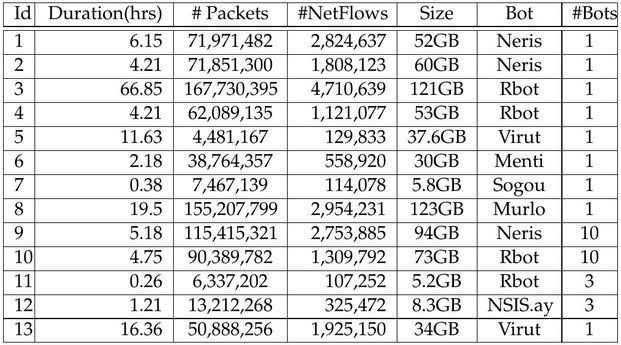
\includegraphics[width=1\textwidth]{Figures/ctu13-2}
\decoRule
\caption[Amount of data and botnet type for each capture]{Amount of data and botnet type for each capture. \cite{garcia2014empirical}}
\label{fig:ctu13-2}
\end{figure}

\noindent Each capture contains only a small amount of botnet samples as seen in Figure~\ref{fig:ctu13-1}.  Most flows are background flows. This is expected of botnet behaviour since it does not generate an large amount of network traffic. The actual labeling is much more detailed as compared to Figure~\ref{fig:ctu13-1}. Each flow is labeled with its exact source. This could be google analytics, google webmail or a windows update. The flows within the dataset only contain the regular information that is found within netflow. The abnormal behaviour within this dataset is internal abnormal behaviour.

 \begin{figure}[H]
\centering
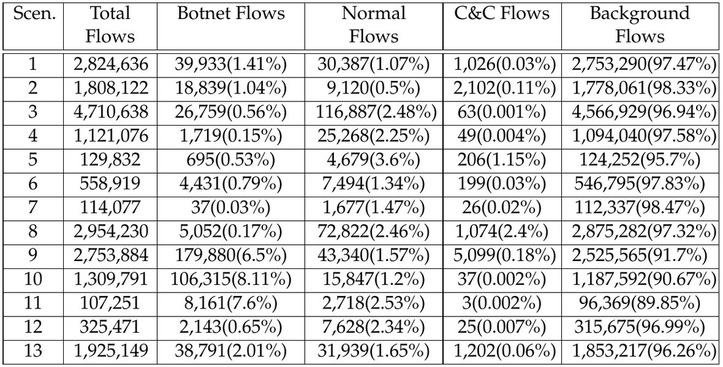
\includegraphics[width=1\textwidth]{Figures/ctu13-1}
\decoRule
\caption[Distribution of labels in CTU 13 Dataset]{Distribution of labels in CTU 13 Dataset. \cite{garcia2014empirical}}
\label{fig:ctu13-1}
\end{figure}

\subsection{Tracelabel Dataset}
This dataset has been used for steps one to three for the testing of the machine learning algorithms. The tracelabel dataset is a database constructed at the University of Twente in September 2008. It contains flow data of traffic collected from a honeypot that was positioned in the network of the university. The honeypot ran sevaral network services such as ftp, ssh, http, etc. The honeypot only captured abnormal behaviour. As such, most of the data within the dataset is actual abnormal behaviour. \cite{sperottoIPOM2009} \\
\\
The flows within the dataset contain extra information. Each flow also contains the TCP flags obtained by OR-ing the TCP flags field of all packets of the flow.  In Table~\ref{tab:tracelabel}, the labeling that is used within this dataset can be seen. The abnormal behaviour within this dataset is external abnormal behaviour. 

\begin{table}[H]
\caption{Labeling of the Tracelabel dataset.}
\label{tab:tracelabel}
\centering
\begin{tabular}{| l | c | r|}
\toprule
\tabhead{Id} & \tabhead{label} & \tabhead{Explanation}\\
\midrule
 1 & ssh\_scan & An ssh scan \\
 2 & ssh\_conn & Unauthorized ssh connection attempt \\
 3 & ftp\_scan & An ftp scan \\
 4 & ftp\_conn & Unauthorized ftp connection attempt \\
 5 & http\_scan & An http scan \\
 6 & http\_conn & Unauthorized http connection attempt \\
 7 & authident\_sideeffect  & Unauthorized identification attempt \\
 8 & irc\_sideeffect  & Suspicious irc traffic \\
 9 & icmp\_sideeffect & Suspicious icmp traffic \\
\bottomrule
\end{tabular}
\end{table}

\subsection{EDM Dataset}
This dataset has been used for step four for the testing of the machine learning algorithms. This is a dataset of unlabeled netflow data gathered from the EDM network. It spans from the 18th of Februari, 2016 till the 24th of March  2016. The data spans from 10am till midnight. This dataset is used mainly to check whether the machine learning algorithms perform well on real-world data.

\subsection{Cegeka Dataset}
A dataset from Cegeka has been used. This dataset spans three days, from the third of April till the  fifth of April. This dataset contains unlabeled netflow data. It also contains logs from firewalls. These logs can be used to check whether the machine learning algorithm has a good performance. 

\section{Feature selection}
A lot of information can be found within a flow as explained in Section~\ref{flow}. The standard attributes of a flow have also been chosen to be used as features. The extra information such as the TCP flags that are set have not been used since they are not available in the datasets that have been used. \\
\\
The country of origin has also been used  in the implementation. However most services that provide such an API are limited in use and cannot be used to request data for millions of flows.

\section{Algorithm selection}
Both supervised and unsupervised algorithms have been used. The algorithms from Section~\ref{algorithms} are the most common algorithms. Before more complex algorithms such as deep neural networks should be used, the more common and general algorithms should be tested. 

\subsection{Unsupervised learning}
K-Means clustering is used in order to test whether results can be found using clustering algorithms. K-means is a simple clustering algorithm and already gives an indication whether a problem can be solved using clustering, or whether clustering offers no advantage. \\
\\
One-class Support Vector machines are used in an attempt to use binary classification. They are quite fast in execution. They were used to find out whether it is a viable technique to preprocess incoming data and check whether a One-class Support Vector machine finds it to be abnormal behaviour before passing it to other algorithms.

\subsection{Supervised learning}
Support vector machines have been used in the implementation. It is an popular algorithm and can do both linear and non-linear classification which make it a promising choice to test in the implementation. \\
\\
K-nearest Neighbors was the most promising algorithm. This algorithm is used extensively through throughout the implementation and the tests. The fact that the classification happens on basis of the different neighbors instead of trying to make a classifier seemed to fit the feature data better. \\
\\
Neural networks also seemed very promising. However, the library \textit{scikit-learn} does not implement neural networks and as such, they have not been used in the implementation. \\
\\
Through the study of different machine learning algorithms, decision tree algorithms and Bayesian algorithms have also been discussed. They seemed less promising for the problem of intrusion detection. The difference between a normal flow and an abnormal flow is very slight and it seemed that these algorithms would make more mistakes. They are still used in the implementation.
